\section{Fields}
\label{sec:fields}

\begin{outcome}
  \begin{enumerate}
  \item Solve systems of equations using scalars from a field other
    than the real numbers, such as $\Z_2$ or $\Z_5$.
  \end{enumerate}
\end{outcome}

So far in this chapter, we have worked with real numbers: all of the
scalars we used, for coefficients, constant terms, variables, and
parameters, were real numbers. But in fact, we have not used very many
properties of the real numbers, except for the fact that we can add,
subtract, multiply, and divide them. For example, we have never needed
to take a square root or to compute a trigonometric function.

In fact, most of linear algebra only requires addition, subtraction,
multiplication, and division. This opens to door to doing linear
algebra using other kinds of scalars besides the real numbers. For
example, we can do linear algebra over the rational numbers, complex
numbers, or even over some more exotic number systems that you will
learn about in this section. A system of scalars that one can do
linear algebra with is called a {\em field}.

\begin{definition}{Field}{field}
  \index{properties of addition!field}%
  \index{properties of multiplication!field}%
  A \textbf{field}\index{field} is a set $F$, together with two
  operations called \textbf{addition}%
  \index{addition!in a field} and
  \textbf{multiplication}%
  \index{multiplication!in a field}, and
  together with two distinct elements $0$ and $1$, such that addition
  and multiplication satisfy the following properties:
  \begin{itemize}
  \item[(A1)] {Commutative law of addition:} $a+b=b+a$;
    \index{commutative law!of addition}%
  \item[(A2)] {Associative law of addition:} $(a+b)+c = a+(b+c)$;
    \index{associative law!of addition}%
  \item[(A3)] {Unit law of addition:} $0+a = a$;
    \index{additive unit}%
  \item[(A4)] {Additive inverse:} for each $a\in F$, there exists an element $(-a)\in F$ such that $a+(-a)=0$;
    \index{additive inverse}%
    \index{inverse!additive}%
  \item[(M1)] {Commutative law of multiplication:} $ab=ba$;
    \index{commutative law!of multiplication}%
  \item[(M2)] {Associative law of multiplication:} $(ab)c=a(bc)$;
    \index{associative law!of multiplication}%
  \item[(M3)] {Unit law of multiplication:} $1a=a$;
    \index{multiplicative unit}\index{unit!of multiplication|see{multiplicative unit}}%
  \item[(M4)] {Multiplicative inverse:} for each non-zero $a\in F$, there exists an element $a^{-1}\in F$ such that $aa^{-1}=1$;
    \index{multiplicative inverse}%
    \index{inverse!multiplicative}%
    \index{inverse!in a field}%
    \index{inverse!modulo p@modulo $p$}%
  \item[(D)] {Distributive law:} $a(b+c)=ab+ac$.
    \index{distributive law!of fields}%
  \end{itemize}
\end{definition}

Properties (A1)--(A4) are about addition, properties (M1)--(M4) are
about multiplication, and property (D) is about both addition and
multiplication. Here are some examples and non-examples of fields:

\begin{example}{Some fields and some non-fields}{fields-examples}
  \begin{enumialphparenastyle}
    \begin{enumerate}
    \item The set $\R$ of real numbers is a field.
    \item The set $\Q$ of rational numbers is a field.
    \item The set $\Z$ of integers satisfies all field
      properties except for (M3). It is therefore not a field.
    \item The set $\N=\set{0,1,2,\ldots}$ of natural numbers
      satisfies all field properties except (A3) and (M3). It is
      therefore not a field.
    \end{enumerate}
  \end{enumialphparenastyle}
\end{example}

A field doesn't have to be infinite. The following is an example of a
field with only two elements.

\begin{example}{The integers modulo 2}{z-mod-2}
  \index{modulo}%
  Consider the set of {\em bits}\index{bit} (binary digits) $\set{0,1}$.
  We can multiply them as usual, and add them almost as usual, subject
  to the alternative rule $1+1=0$ (instead of $1+1=2$). Here is a
  summary of the rules for addition and multiplication:
  \begin{equation*}
    \begin{array}{l|ll}
      +&0&1 \\\hline
      0&0&1 \\
      1&1&0
    \end{array}
    \quad
    \begin{array}{l|ll}
      \cdot&0&1 \\\hline
      0&0&0 \\
      1&0&1
    \end{array}
  \end{equation*}
  This particular alternative arithmetic is called ``arithmetic modulo
  2''.  In computer science, the addition is also called the ``logical
  exclusive or'' operation\index{logical operation!exclusive or}, and
  multiplication is also called the ``logical and''
  operation\index{logical operation!and}. You can also think of $0$ as
  ``even'' and $1$ as ``odd'', and not that odd plus odd makes
  even. For example, we can calculate like this:
  \begin{equation*}
    \begin{array}{lll}
      1\cdot((1+0)+1) + 1 &=& 1\cdot(1+1) + 1\\
                          &=& 1\cdot 0 + 1\\
                          &=& 0 + 1\\
                          &=& 1.
    \end{array}
  \end{equation*}
  The binary digits form a field $\Z_2 = \set{0,1}$, also
  called \textbf{the field of integers modulo 2}\index{integers modulo $p$}.
\end{example}

You can convince yourself that the 9 properties of fields are all
satisfied by the integers modulo 2. This is a bit tedious, but it can
be checked by calculations.  For example, to verify (A1), we have to
check that $0+0=0+0$, $0+1=1+0$, $1+0=0+1$, and $1+1=1+1$. Perhaps the
most interesting properties are (A4) and (M4). For (A4), we can set
$(-0)=0$ and $(-1)=1$. It may be surprising that $(-1)=1$, but you can
check for yourself that $1+(-1)=1+1=0$ when calculating modulo
$2$. For (M4), we can set $1^{-1} = 1$.

When solving systems of linear equations, we only used addition,
subtraction, multiplication, and division. Therefore, we can solve
systems of equations using the elements of any field as the scalars,
instead of the real numbers.

\begin{example}{Solving a system of equations over $\Z_2$}{system-z2}
  Solve the following system in the integers modulo 2:
  \begin{equation*}
    \begin{array}{r@{~}c@{~}l}
      x + y     &=& 0 \\
      x     + z &=& 1 \\
          y + z &=& 1.
    \end{array}
  \end{equation*}
\end{example}

\begin{solution}
  As usual, we write the augmented matrix of the system of equations,
  then reduce it to {\rref} using elementary row operations. The only
  difference is that we will perform all arithmetic operations modulo
  2, rather than in the real numbers. The augmented matrix is:
  \begin{equation*}
    \begin{mymatrix}{rrr|r}
      1 & 1 & 0 & 0 \\
      1 & 0 & 1 & 1 \\
      0 & 1 & 1 & 1 \\
    \end{mymatrix}.
  \end{equation*}
  The first pivot entry is the $1$ in the upper left. We use a row
  operation to create a zero below it. Note that, because we are
  working modulo 2, adding $1$ and subtracting $1$ is the same thing.
  \begin{equation*}
    \begin{mymatrix}{rrr|r}
      \circled{1} & 1 & 0 & 0 \\
      1 & 0 & 1 & 1 \\
      0 & 1 & 1 & 1 \\
    \end{mymatrix}
    \stackrel{R_2\rowop R_2+R_1}{\sim}
    \begin{mymatrix}{rrr|r}
      \circled{1} & 1 & 0 & 0 \\
      0 & 1 & 1 & 1 \\
      0 & 1 & 1 & 1 \\
    \end{mymatrix}.
  \end{equation*}
  The next pivot entry is in row 2 and column 2. We create a zero
  below it by subtracting row 2 from row 3, and a zero above it by
  subtracting row 2 from row 1:
  \begin{equation*}
    \begin{mymatrix}{rrr|r}
      \circled{1} & 1 & 0 & 0 \\
      0 & \circled{1} & 1 & 1 \\
      0 & 1 & 1 & 1 \\
    \end{mymatrix}
    \stackrel{R_3\rowop R_3-R_2}{\sim}
    \begin{mymatrix}{rrr|r}
      \circled{1} & 1 & 0 & 0 \\
      0 & \circled{1} & 1 & 1 \\
      0 & 0 & 0 & 0 \\
    \end{mymatrix}
    \stackrel{R_1\rowop R_1-R_2}{\sim}
    \begin{mymatrix}{rrr|r}
      \circled{1} & 0 & 1 & 1 \\
      0 & \circled{1} & 1 & 1 \\
      0 & 0 & 0 & 0 \\
    \end{mymatrix}.
  \end{equation*}
  The resulting system is in {\rref}. We can see that the system is
  consistent, because there is no row whose left-hand side is zero and
  whose right-hand side is non-zero. We also see that there are two
  pivot columns, and therefore two pivot variables, $x$ and $y$. On
  the other hand, $z$ is a free variable, so we set it equal to a
  parameter: $z=t$. Notice that this time, the parameter $t$ is not a
  real number, but an element of $\Z_2$. From the equation
  $x+z=1$, we get $x=1-z=1+t$. Can you guess why I have written $1+t$
  instead of $1-t$? This is because $(-1)=1$ in the integers modulo 2.
  So $1-t = 1+(-1)t = 1+1t = 1+t$. Similarly, from the equation
  $y+z=1$, we get that $y=1+t$. Therefore, the general solution to the
  system of equations is
  \begin{equation*}
    \begin{array}{r@{~}c@{~}l}
      x &=& 1+t \\
      y &=& 1+t \\
      z &=& t,
    \end{array}
  \end{equation*}
  where $t\in\set{0,1}$ is an arbitrary parameter. Recall that this
  means that each time we plug in a particular value for $t$, we get a
  solution.

  There is one difference between solving equations in the real
  numbers and solving equations in $\Z_2$. In the real
  numbers, a system of equations has either no solution, a unique
  solution, or infinitely many solutions. This is because when there
  is a parameter, we automatically get infinitely many solutions. By
  contrast, in $\Z_2$, there are only two scalars, and
  therefore only two possible values for the parameter $t$, namely
  $t=0$ and $t=1$. For $t=0$ we get the solution $(x,y,z) = (1,1,0)$,
  and for $t=1$ we get the solution $(x,y,z) = (0,0,1)$.  Thus, when
  the general solution has one parameter in $\Z_2$, there are
  only two solutions, instead of infinitely many.
\end{solution}

\begin{example}{A game with buttons and lights}{button-game}
  Consider a game with 9 lights arranged in a square:
  \begin{center}
    \begin{tabular}{|c|c|c|}
      \hline
      \rule{0ex}{8.5mm}
\includegraphics[width=7mm]{figures/lighton} &
      \rule{0ex}{8.5mm}
\includegraphics[width=7mm]{figures/lightoff} &
      \rule{0ex}{8.5mm}
\includegraphics[width=7mm]{figures/lighton} \\\hline 
      \rule{0ex}{8.5mm}
\includegraphics[width=7mm]{figures/lightoff} &
      \rule{0ex}{8.5mm}
\includegraphics[width=7mm]{figures/lighton} &
      \rule{0ex}{8.5mm}
\includegraphics[width=7mm]{figures/lightoff} \\\hline 
      \rule{0ex}{8.5mm}
\includegraphics[width=7mm]{figures/lightoff} &
      \rule{0ex}{8.5mm}
\includegraphics[width=7mm]{figures/lightoff} &
      \rule{0ex}{8.5mm}
\includegraphics[width=7mm]{figures/lighton} \\\hline 
    \end{tabular}
  \end{center}
  Each light is also a button. When a button is pressed, its own
  light, and all the lights neighboring it (i.e., above, below, to the
  left and to the right) are toggled (i.e., any light that was off is
  turned on and vice versa). Figure out which buttons to press to
  turn off all the lights if the starting position is as shown above.
\end{example}

\begin{solution}
  We number the lights and buttons from top to bottom, left to right,
  like this:
  \begin{center}
    \begin{tabular}{|c|c|c|}
      \hline
      1 & 2 & 3 \\\hline
      4 & 5 & 6 \\\hline
      7 & 8 & 9 \\\hline
    \end{tabular}.
  \end{center}
  Let $x_i$ be a variable in $\Z_2$, corresponding to the
  event ``button $i$ is pressed'' (or more precisely, ``button $i$
  is pressed an odd number of times'', because pressing a button
  twice is the same as not pressing it at all. That is why we are
  working modulo 2). To turn off the light at position 1, we must
  press an odd number of buttons 1, 2, and 4. In other words,
  $x_1+x_2+x_4 = 1$. To ensure the light at position 2 stays off, we
  must press an even number of buttons 1, 2, 3, and 5, or as an
  equation, $x_1+x_2+x_3+x_5=0$. In this way, we obtain 9 linear
  equations in 9 variables:
  \begin{equation*}
    \begin{array}{r@{~}c@{~}l}
      x_1+x_2+x_4 &=& 1 \\
      x_1+x_2+x_3+x_5 &=& 0 \\
      x_2+x_3+x_6 &=& 1 \\
      x_1+x_4+x_5+x_7 &=& 0 \\
      x_2+x_4+x_5+x_6+x_8 &=& 1 \\
      x_3+x_5+x_6+x_9 &=& 0 \\
      x_4+x_7+x_8 &=& 0 \\
      x_5+x_7+x_8+x_9 &=& 0 \\
      x_6+x_8+x_9 &=& 1.
    \end{array}
  \end{equation*}
  Here is the augmented matrix for the system:
  \begin{equation*}
    \begin{mymatrix}{rrrrrrrrr|r}
      1&1&0 & 1&0&0 & 0&0&0 & 1 \\
      1&1&1 & 0&1&0 & 0&0&0 & 0 \\
      0&1&1 & 0&0&1 & 0&0&0 & 1 \\
      
      1&0&0 & 1&1&0 & 1&0&0 & 0 \\
      0&1&0 & 1&1&1 & 0&1&0 & 1 \\
      0&0&1 & 0&1&1 & 0&0&1 & 0 \\
      
      0&0&0 & 1&0&0 & 1&1&0 & 0 \\
      0&0&0 & 0&1&0 & 1&1&1 & 0 \\
      0&0&0 & 0&0&1 & 0&1&1 & 1 \\
    \end{mymatrix}.
  \end{equation*}
  We solve this system of equations by doing Gauss-Jordan
  elimination with scalars in $\Z_2$.  The {\rref} is
  \begin{equation*}
    \begin{mymatrix}{rrrrrrrrr|r}
      1&0&0 & 0&0&0 & 0&0&0 & 0 \\
      0&1&0 & 0&0&0 & 0&0&0 & 0 \\
      0&0&1 & 0&0&0 & 0&0&0 & 1 \\
      
      0&0&0 & 1&0&0 & 0&0&0 & 1 \\
      0&0&0 & 0&1&0 & 0&0&0 & 1 \\
      0&0&0 & 0&0&1 & 0&0&0 & 0 \\
      
      0&0&0 & 0&0&0 & 1&0&0 & 0 \\
      0&0&0 & 0&0&0 & 0&1&0 & 1 \\
      0&0&0 & 0&0&0 & 0&0&1 & 0 \\
    \end{mymatrix}.
  \end{equation*}
  This means we have to press buttons 3, 4, 5, and 8. Also, since
  the rank is 9, the solution is unique.
\end{solution}

\begin{example}{The integers modulo 5}{z-mod-5}
  Consider the set $\Z_5=\set{0,1,2,3,4}$, called the
  \textbf{integers modulo 5}\index{integers modulo $p$}. We define their
  addition and multiplication by computing the usual addition and
  multiplication, then ``reducing'' the answer modulo 5. Here,
  ``reducing'' a number means repeatedly subtracting 5 until the
  answer is between $0$ and $4$. Imagine a clock showing 5 numbers
  instead of the usual 12:
  \begin{center}
    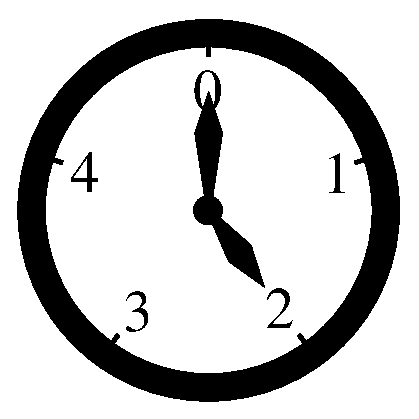
\includegraphics[width=2.5cm]{figures/clock}
  \end{center}
  If we want to calculate 3 o'clock plus 4 hours, we get 2 o'clock,
  because whenever the clock reaches 5, it resets to 0. This is how
  addition and multiplication modulo 5 are defined:
  \begin{equation*}
    \begin{array}{l|lllll}
      +&0&1&2&3&4 \\\hline
      0&0&1&2&3&4 \\
      1&1&2&3&4&0 \\
      2&2&3&4&0&1 \\
      3&3&4&0&1&2 \\
      4&4&0&1&2&3 \\
    \end{array}
    \quad
    \begin{array}{l|lllll}
      \cdot&0&1&2&3&4 \\\hline
      0&0&0&0&0&0 \\
      1&0&1&2&3&4 \\
      2&0&2&4&1&3 \\
      3&0&3&1&4&2 \\
      4&0&4&3&2&1 \\
    \end{array}
  \end{equation*}
\end{example}

We note that the integers modulo 5 form a field. Most of the
properties are tedious but easy to verify. Perhaps the most
interesting of the field properties is (M4). It says that for each
non-zero element $a$, there is another element $a^{-1}$ such that
$aa^{-1}=1$.  By looking at the multiplication table, we see that
$1\cdot 1=1$, $2\cdot 3=1$, $3\cdot 2=1$, and $4\cdot 4=1$. Therefore
we can set $1^{-1}=1$, $2^{-1}=3$, $3^{-1}=2$, and $4^{-1}=4$.

\begin{example}{Division in $\Z_5$}{division-z5}
  What is 2 divided by 3 in $\Z_5$?
\end{example}

\begin{solution}
  There are no fractions in $\Z_5$. The key to dividing is
  this: instead of dividing by $a$, multiply by $a^{-1}$. So we have:
  \begin{equation*}
    2/3 = 2\cdot 3^{-1} = 2\cdot 2 = 4.
  \end{equation*}
  So 2 divided by 3 equals 4. This makes sense, because 4 times 3
  equals 2, when calculating modulo 5.
\end{solution}

\begin{example}{Solving a system of equations over $\Z_5$}{system-z5}
  Solve the following system of linear equations over $\Z_5$:
  \begin{equation*}
    \begin{array}{r@{~}c@{~}l}
      2x + z &=& 1 \\
      x+4y+z &=& 3 \\
      x+2y+3z &=& 2. \\
    \end{array}
  \end{equation*}
\end{example}

\begin{solution}
  We perform the usual Gauss-Jordan algorithm on the augmented
  matrix. The only thing to keep in mind is that, instead of dividing
  a row by $a$, we should multiply it by $a^{-1}$. And of course, we
  should reduce all intermediate results modulo $5$. For example, to
  change the first pivot entry from $2$ to $1$, we multiply by
  $2^{-1}=3$, instead of dividing by $2$.
  \begin{equation*}
    \begin{mymatrix}{rrr|r}
      \circled{2} & 0 & 1 & 1 \\
      1 & 4 & 1 & 3 \\
      1 & 2 & 3 & 2
    \end{mymatrix}
    \stackrel{R_1\rowop 3R_1}{\sim}
    \begin{mymatrix}{rrr|r}
      \circled{1} & 0 & 3 & 3 \\
      1 & 4 & 1 & 3 \\
      1 & 2 & 3 & 2
    \end{mymatrix}
    \stackrel{R_2\rowop R_2-R_1}{\stackrel{R_3\rowop R_3-R_1}{\sim}}
    \begin{mymatrix}{rrr|r}
      \circled{1} & 0 & 3 & 3 \\
      0 & \circled{4} & 3 & 0 \\
      0 & 2 & 0 & 4
    \end{mymatrix}
    \stackrel{R_2\rowop 4R_2}{\sim}
    \begin{mymatrix}{rrr|r}
      \circled{1} & 0 & 3 & 3 \\
      0 & \circled{1} & 2 & 0 \\
      0 & 2 & 0 & 4
    \end{mymatrix}
  \end{equation*}
  \begin{equation*}
    {}
    \stackrel{R_3\rowop R_3-2R_2}{\sim}
    \begin{mymatrix}{rrr|r}
      \circled{1} & 0 & 3 & 3 \\
      0 & \circled{1} & 2 & 0 \\
      0 & 0 & \circled{1} & 4
    \end{mymatrix}
    \stackrel{R_1\rowop R_1-3R_3}{\stackrel{R_2\rowop R_2-2R_3}{\sim}}
    \begin{mymatrix}{rrr|r}
      \circled{1} & 0 & 0 & 1 \\
      0 & \circled{1} & 0 & 2 \\
      0 & 0 & \circled{1} & 4
    \end{mymatrix}.
  \end{equation*}
  The final matrix is in {\rref}, and we see that the system has the
  unique solution $(x,y,z) = (1,2,4)$. Please double-check the
  solution with respect to the original equations.
\end{solution}

\begin{example}{The integers modulo 6 are not a field}{nofield-z6}
  Do the integers modulo 6 form a field? 
\end{example}

\begin{solution}
  The integers modulo 6 are the set $\Z_6=\set{0,1,2,3,4,5}$, with the
  addition and multiplication modulo 6:
  \begin{equation*}
    \begin{array}{l|llllll}
      +&0&1&2&3&4&5 \\\hline
      0&0&1&2&3&4&5 \\
      1&1&2&3&4&5&0 \\
      2&2&3&4&5&0&1 \\
      3&3&4&5&0&1&2 \\
      4&4&5&0&1&2&3 \\
      5&5&0&1&2&3&4 \\
    \end{array}
    \quad
    \begin{array}{l|llllll}
      +&0&1&2&3&4&5 \\\hline
      0&0&0&0&0&0&0 \\
      1&0&1&2&3&4&5 \\
      2&0&2&4&0&2&4 \\
      3&0&3&0&3&0&3 \\
      4&0&4&2&0&4&2 \\
      5&0&5&4&3&2&1 \\
    \end{array}
  \end{equation*}
  Then $\Z_6$ satisfies all of the field axioms except
  (M3). To see why (M3) fails, let $a=2$, and note, by looking at the
  multiplication table, that there is no $b\in\Z_6$ such that
  $ab=1$. Therefore, $\Z_6$ is not a field.
\end{solution}

We conclude this section with a fact that we will not prove.

\begin{theorem}{The integers modulo a prime}{z-mod-p}
  Let $n$ be a positive integer. Then the set
  $\Z_n=\set{0,\ldots,n-1}$ of integers modulo $n$, with
  addition and multiplication modulo $n$, forms a field if and only if
  $n$ is prime. Thus, for example, $\Z_2$, $\Z_3$,
  $\Z_5$, $\Z_7$, and $\Z_{11}$ are fields,
  whereas $\Z_4$, $\Z_6$, and $\Z_9$ are not.
\end{theorem}
